\documentclass{beamer}
\begin{document}
\title{Python Chapter 1}
\author{Ezequiel Torres}
\date{\today}
\frame{\titlepage}
\frame{\frametitle{Table of contents}\tableofcontents}

\section{Section no.1}
\frame{\frametitle{Before getting started}
    We will be going over the basics of python and interviewing in python in this course.
    Here are some great resources to get started.
    \begin{itemize}
        \item<1-> http://programarcadegames.com
            \begin{itemize}
                \item<2-> Fun way to learn python at your own pace while making arcade games!
            \end{itemize}
        \item<3-> https://www.crackingthecodinginterview.com/
            \begin{itemize}
                \item<4-> 
\includegraphics{CTCI.png}
            \end{itemize}
    \end{itemize}
}
\frame{\frametitle{Before getting started}
    \begin{itemize}
        \item<1-> 
            \begin{itemize} https://www.amazon.com/Grokking-Algorithms-illustrated-programmers-curious/dp/1617292230
                \item<2-> 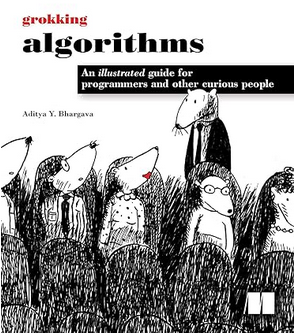
\includegraphics{ga.png}
            \end{itemize}
        \item<3-> https://www.crackingthecodinginterview.com/
            \begin{itemize}
                \item<4-> 
\includegraphics{CTCI.png}
            \end{itemize}
    \end{itemize}
}


\section{Section no.2}
\frame{\frametitle{Variables} 
    Here we will go into some basic examples of variables in python.
    \begin{enumerate}
        \item basic item
    \end{enumerate}
}


\end{document}
